%%%%%%%%%%%%%%%%%%%%%% Props %%%%%%%%%%%%%%%%%%%%%%
\documentclass{article}

\usepackage[french]{babel}
\usepackage[utf8]{inputenc}
\usepackage[T1]{fontenc}
\usepackage{graphicx}
\usepackage{fancyhdr}
\usepackage{eurosym}
\usepackage{color}
\usepackage{soul}
\usepackage{listings}
\usepackage{enumitem}
\usepackage{enumerate}

\pagestyle{fancy}
\lhead{Soutenance 3}
\chead{Deadly Science}
\rhead{Custos Carceris}

\definecolor{mygreen}{rgb}{0,0.6,0}
\definecolor{mygray}{rgb}{0.5,0.5,0.5}
\definecolor{mymauve}{rgb}{0.58,0,0.82}

\lstset{ 
  commentstyle=\color{mygreen},
  keywordstyle=\color{blue},       % keyword style
  numberstyle=\tiny\color{mygray}, % the style that is used for the line-numbers
  rulecolor=\color{black},         % if not set, the frame-color may be changed on line-breaks within not-black text (e.g. comments (green here))
  stringstyle=\color{mymauve},     % string literal style
  language=[Sharp]C,                 % the language of the code
  backgroundcolor=\color{white},   % choose the background color; you must add \usepackage{color} or \usepackage{xcolor}; should come as last argument
  basicstyle=\footnotesize,        % the size of the fonts that are used for the code
  breakatwhitespace=true,         % sets if automatic breaks should only happen at whitespace
  breaklines=true,
  extendedchars=true,              % lets you use non-ASCII characters; for 8-bits encodings only, does not work with UTF-8
  frame=single,	                   % adds a frame around the code
  tabsize=2,	                   % sets default tabsize to 2 spaces
  showstringspaces=false,
  numbers=left,
}

\begin{document}


%%%%%%%%%%%%%%%%%%%%%% Titre %%%%%%%%%%%%%%%%%%%%%%
\begin{titlepage}
	\centering
	{\scshape\LARGE Custos Carceris\par}
	\vspace{1cm}
	{\scshape\Large Rapport de projet\par}
	\vspace{1.5cm}
	{\huge\bfseries Deadly Science\par}
	\vspace{2cm}
	
\includegraphics[width=0.5\textwidth]{logo.png}\par\vspace{1cm}
	{\Large\itshape Léandre Perrot\par}
	{\Large\itshape Yann Boudry\par}
	{\Large\itshape Steve Suissa\par}
	{\Large\itshape Célian Raimbault\par}
	\vfill
	Un projet EPITA
	\vfill
	{\large \today\par}
\end{titlepage}



\newpage
\tableofcontents


%%%%%%%%%%%%%%%%%%%%% Intro %%%%%%%%%%%%%%%%%%%%%%

\newpage
\section{Introduction}

%%%%%%%%%%%%%%% TODO : Mettre a jour
Le jeu a grandement avancé depuis le retour du cahier des charges : le réseau est quasiment entièrement fonctionnel, pareil pour la caméra, le site avance petit à petit, la génération est presque fini et certaines musiques ont été composées. Globalement, le jeu est quasiment jouable.
\begin{table}[!h]
\centering
\caption{Avancement}
\begin{tabular}{|l|l|l|}

\hline
%%%%%%%%%%%%%%% TODO : Mettre a jour
Tâches $\backslash$Soutenances & Attendu & Réalité \\ \hline
Camera & 50\% & 75\% \\ \hline
G Joueur & 30\% & 50\% \\ \hline
G Jeu & 30\% & 30\% \\ \hline
Reseau & 50\% & 75\% \\ \hline
Map Const & 30\% & 30\% \\ \hline
Menu & 15\% & 70\% \\ \hline
Chrono/GUI & 30\% & 30\% \\ \hline
Site TXT & 0\% & 30\% \\ \hline
Site E & 0\% & 0\% \\ \hline
Map Gen & 0\% & 50\% \\ \hline
Musique & 0\% & 25\% \\ \hline
Sons & 0\% & 10\% \\ \hline

\end{tabular}
\end{table}
 
\newpage
\section{Reprise du cahier des charges}
blablabla
\newpage
\section{Présentation du projet}



\subsection{Menus}
blablabla
%%%%%%%%%%%%%%%%%%%%%% Yann %%%%%%%%%%%%%%%%%%%%%%%%%%%%%%
\subsubsection{Menu principal}
blablabla
\newpage
\subsubsection{Menus de connection}
%%%%%%%%%%%%%%%%%%%%%% Steve%%%%%%%%%%%%%%%%%%%%%%%%%%%%%%
Pour se connecter il y'a trois menus, le menu pour créer la partie, le menu pour changer les paramètres de la partie, et enfin le menu on peut voir les joueurs connectés et commencer la partie. Chacun des 3 menus ont subi une refonte graphique pour correspondre à l'ambiance du jeu et avoir un aspect visuel plus plaisant.

\paragraph{Menu pour créer la partie}

Voici à quoi ce menu ressemble : 

\begin{figure}[!ht]
    \centering
    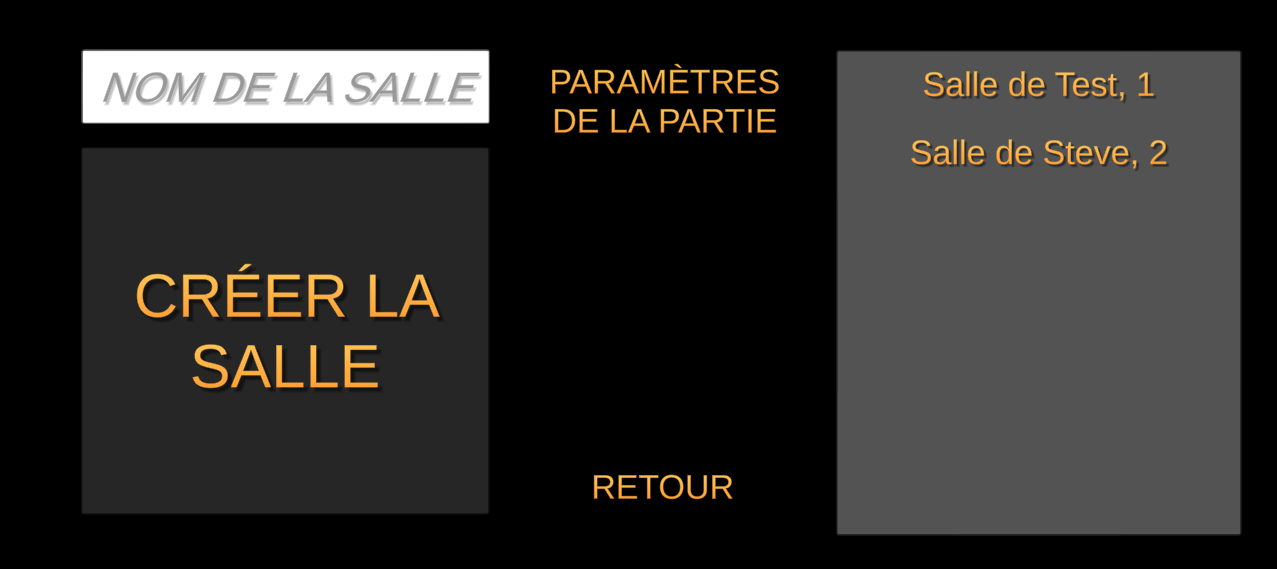
\includegraphics[width=0.8\textwidth]{Menu1.png}
    \caption{Menu pour créer la salle}
    \label{Menu pour créer la salle}
\end{figure}

Il est composé de deux parties. Celle de gauche on peut écrire dans la barre blanche le nom de la salle que l'on veut créer et un bouton "Créer la salle" qui comme son nom l'indique permet de créer la salle et d'entrer dans un autre menu que l'on verra par la suite. La partie droite liste chacune des salles avec leur noms et le nombre de joueurs déjà présents dans la salle. Elle est sur un tableau défilant ce qui permet d'avoir autant de parties que l'on souhaite. Cela permet de savoir si par exemple on va attendre plus ou moins longtemps avant le début de la partie. Pour rejoindre la salle que l'on souhaite, c'est simple, il suffit de cliquer dessus et cela nous fait rentrer dans la dite salle. A noter que si la salle est remplie à son maximum, elle ne sera pas montrée comme visible, vu qu'on ne peut pas la rejoindre. En ce qui concerne les deux boutons du milieu, le bouton "Retour" nous fait retourner à l'écran principal et le deuxième bouton nous transporte dans le menu des paramètres du labyrinthe que l'on va maintenant regarder.

\paragraph{Menu pour les paramètres de la partie}

Dans ce menu on peut changer de mode de jeu entre Classique et Nocturne (ces modes de jeu seront expliqués par la suite). On peut aussi changer le nombre de joueurs de la partie. Enfin on peut choisir la taille du labyrinthe parmis plusieurs dimensions prédéfinies ou bien choisir une taille personnalisée (par exemple un labyrinthe rectangulaire) en l'écrivant sur la barre blanche et confirmer. Pour sélectionner l'option que l'on souhaite, il suffit encore tout simplement de cliquer dessus. Par exemple sur la Figure 2, on peut voir que le mode de jeu choisi est Classique, que la salle peut contenir quatre joueurs et que la taille du labyrinthe est de dix en largeur et 10 en longueur. Lorsque l'on a choisi ses paramètres, il suffit d'appuyer sur le bouton "Retour" qui nous envoie sur le menu précédant et on peut créer la partie avec les paramètres enregistrés. On peut souligner que les modes de jeu et les tailles du labyrinthe sont sur des tableaux défilants, ce qui permet premièrement l'ajout de nouveaux modes ou de nouvelles tailles facile, mais aussi que l'on peut en ajouter autant qu'on veut, il suffit juste d'utiliser la molette de la sourie pour accéder aux options tout en bas.



\begin{figure}[!ht]
    \centering
    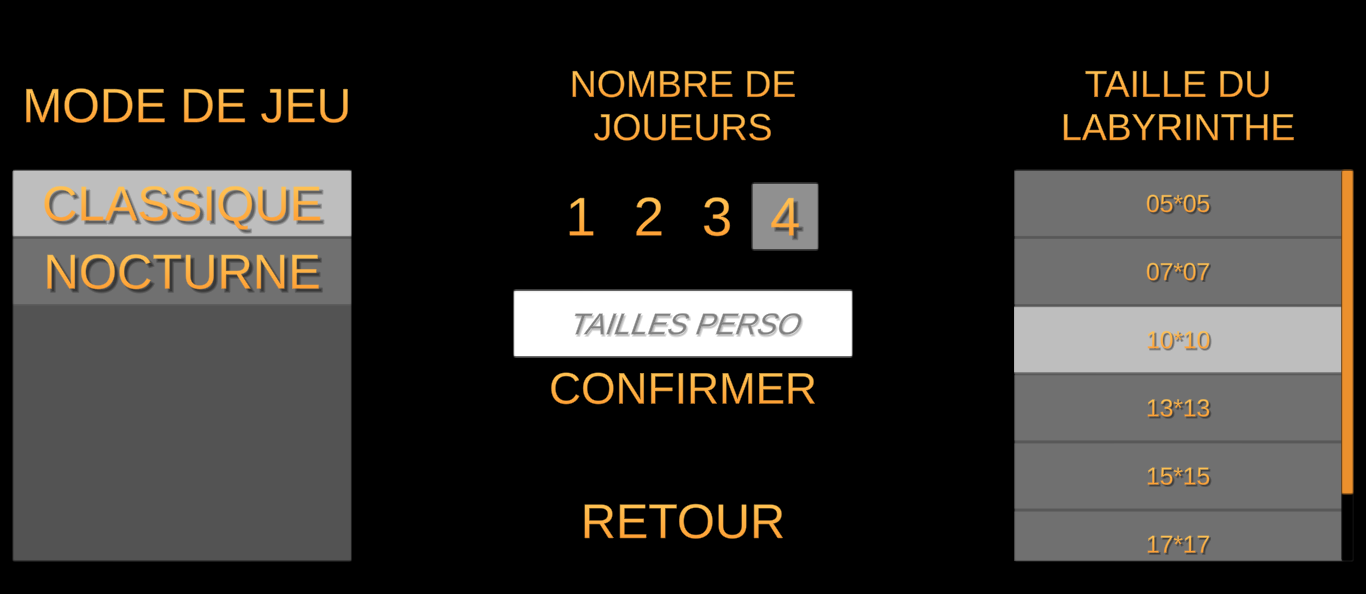
\includegraphics[width=0.8\textwidth]{Menu2.png}
    \caption{Menu pour les paramètres de la partie}
    \label{Menu pour les paramètres de la partie}
\end{figure}


\paragraph{Menu pour commencer la partie}

Ce menu a la particuliarité d'être différend en fonction de notre rôle dans la partie. Si on est l'hôte de la salle, alors le bouton en bas à gauche est "Commencer" permettant de débuter la partie, et sinon il est nommé "Prêt" qui permet de savoir si chacun des joueurs est prêt à commencer la partie comme montré sur les Figures 3 et 4. D'ailleurs à droite, on peut voir la liste des joueurs avec leur pseudonyme et leur rôle. A nôter que l'actualisation des statuts des joueurs est quasiment instantané et que le bouton "Prêt" change si on est prêt ou pas. Si on ne l'est pas il sera renommé "Non Prêt". L'hôte ne peut commencer la partie que si chacun des joueurs, et chacun des joueurs entre dans la salle avec un statut "Non Prêt". Dès que le nombre de joueurs attendus correspond au nombre de joueurs dans la salle et que tous les joueurs sont prêts, l'hôte peut débuter la partie. Lorsque la partie commence, la salle n'est plus accésible ni visible. En dehors de ça, peu importe notre rôle, on peut décider à tout moment de quitter la salle en appuyant sur le bouton éponyme. Si l'on est hôte, tous les joueurs de la salle sont transportés dans le menu pour créer la salle. De plus, des protections ont été mises de manière à ce que même si, par exemple, l'hôte viendrait à cliquer sur le bouton "	Commencer" alors que tous les joueurs ne sont pas prêts, la partie ne débutera pas.

\newpage
\begin{figure}[!ht]
    \centering
    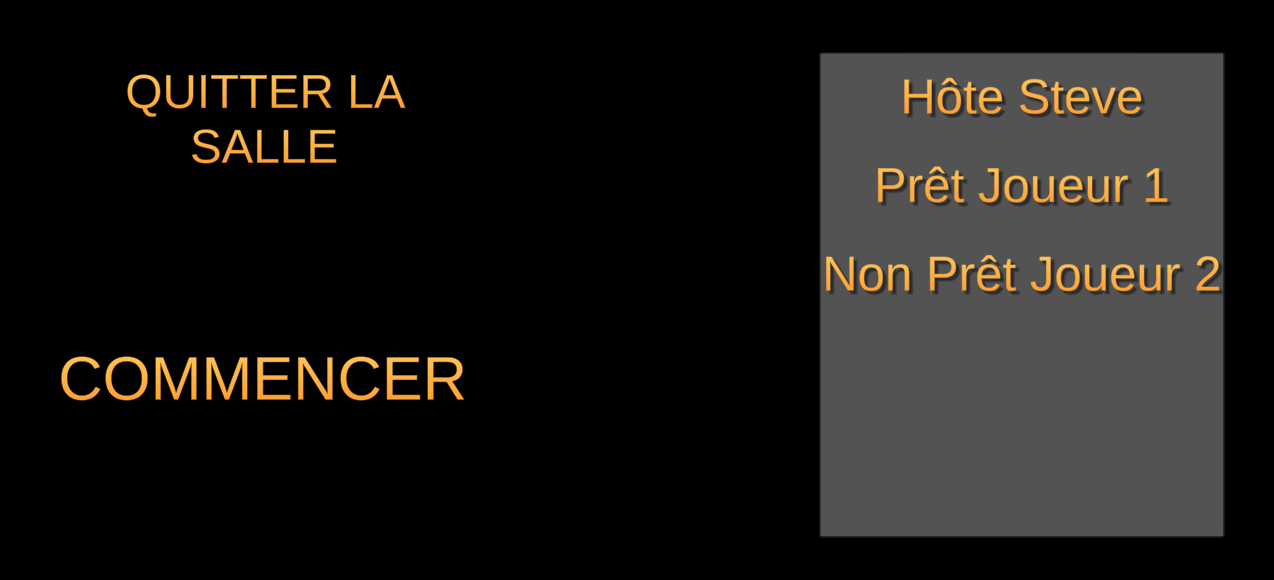
\includegraphics[width=0.8\textwidth]{Menu31.png}
    \caption{Menu lorsqu'on est hôte}
    \label{Menu lorsqu'on est hôte}
\end{figure}



\begin{figure}[!ht]
    \centering
    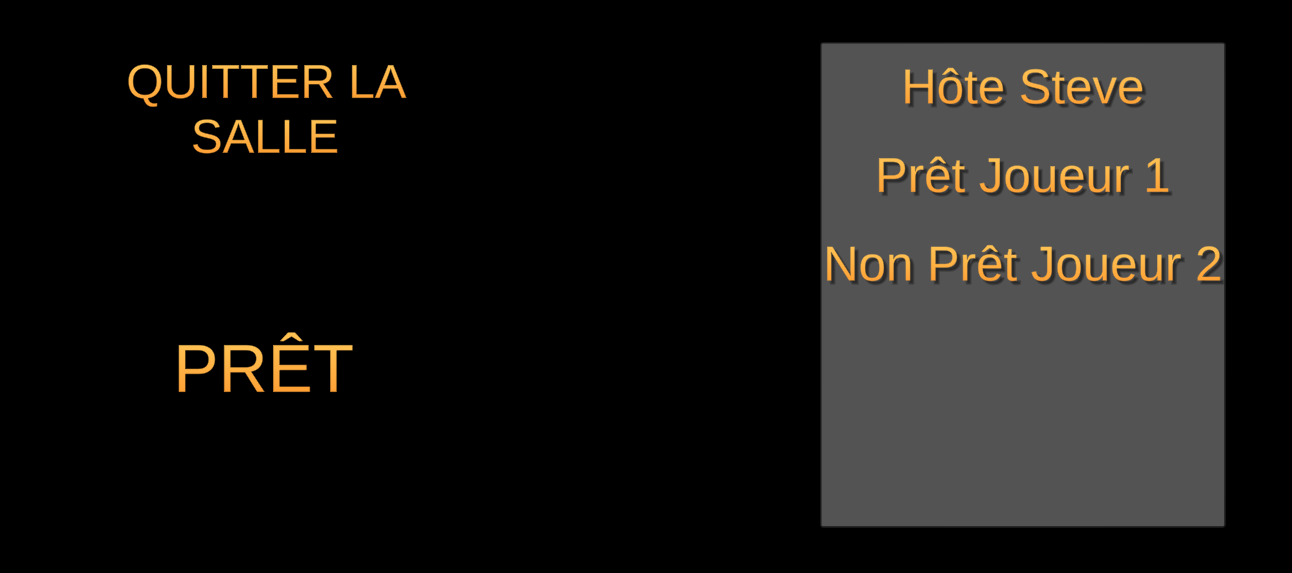
\includegraphics[width=0.8\textwidth]{Menu32.png}
    \caption{Menu lorsqu'on n'est pas hôte}
    \label{Menu lorsqu'on n'est pas hôte}
\end{figure}


\paragraph{Interface}
blablabla
\subsection{Gameplay}
blablabla
\subsubsection{Joueur}
%%%%%%%%%%%%%%%%%%%%%% Celian %%%%%%%%%%%%%%%%%%%%%%%%%%%%%%
blablabla
\subsubsection{Power-Up}
%%%%%%%%%%%%%%%%%%%%%% Léandre %%%%%%%%%%%%%%%%%%%%%%%%%%%%%%
blablabla
\subsection{Labyrinthe}
blablabla
\subsubsection{Partie de Léandre}

Au début du projet, il a été décidé que je serais le responsable de l'ensemble des éléments aléatoires du jeu, ainsi que de la direction artistique. J'ai ainsi commencé en mettant au point un algorithme permettant de générer un dédale de telle sorte que l'ensemble des salles soit accessibles, et que pour accéder à une salle à partir d'un endroit du labyrinthe, il y ait plusieurs itinéraires. L'algorithme a été développé en faisant en sorte qu'il n'y ait aucune sortie, et que l'on puisse modifier la taille du labyrinthe. Au final, l'algorithme correspond à peu de choses près à l'algorithme de Prim, excepté le fait que le nombre d'impasse est nettement moins important. A côté de cette fonction, j'ai également créé une seconde fonction retournant une liste d'entiers aléatoires distincts dans un intervalle donné.

A partir de cet algorithme, on obtient donc une liste dont les valeurs correspondent directement aux passages de chaque "case" du labyrinthe. Pour vérifier que l'algorithme fonctionnait bien, et vite, j'ai mis au point une petite fonction qui se charge d'afficher la carte du labyrinthe ainsi formé dans une console. Après de nombreux tests, aucours desquels j'ai modifié la taille du dédale pour obtenir des configurations rectangulaires, cubiques, voire linéaires pour vérifier le bon fonctionnement de l'algorithme, j'ai transposé le tout sur Unity. J'ai alors modifié la fonction d'affichage en faisant en sorte qu'à la place de mettre des caractères dans une console, Unity instancie des cubes dans une "Scène" prévue à cet effet.

Ensuite, étant donné que nous souhaitions donner à l'ensemble une structure évoquant plus un laboratoire souterrain qu'un jeu de cube pour enfants, j'ai développé une autre fonction pour afficher non pas les murs séparément, mais directement des modèles 3D de salles avec les passages, pour simuler un vrai labyrinthe. La difficulté était ici de bien configurer pour chaque salle l'orientation, ainsi que la position au sein du labyrinthe. Mais j'ai tout de même conservé l'affichage en bloc en vue d'autres tests de génération de l'algorithme, étant donné que cet affichage permet de vérifier plus aisément que la carte du labyrinthe soit valable. Les modèles 3D que j'ai utilisé étaient surtout là pour simuler la carte dans un labyrinthe, et pour effectuer des tests en multijoueur.

A partir de là, on obtient donc un labyrinthe correct, bien que dénué de décorations évoquant un laboratoire. Mais bien qu'il y ait un format correct, ce n'était pas encore jouable : il manquait bien sûr les Sérums et les Joueurs. Concernant les Joueurs, Célian a implémenté une rampe permettant de monter pour sauter directement dans le complexe. En revanche pour les sérums, il nous fallait prendre en compte plusieurs facteurs. Premièrement, un Sérum ne devait pas être implémenté à l'intérieur d'un autre Sérum. Deuxièmement, un Joueur ne devait pas être iinstancié au même emplacement qu'un Sérum, pour éviter qu'un Joueur ne se retrouve infecté dès le début de la partie. Pour cela, j'ai réutilisé la fonction permettant d'obtenir une liste d'entiers aléatoires distincts. Avec cette fonction, il m'était en effet possible d'isoler sept "cases" du complexe dans lesquelles seraient respectivement implémentés les quatres joueurs et les trois sérums. Ainsi, au lancement du jeu, j'ai fait en sorte que le joueur génère les sérums à l'emplacement souhaité. Pour les Sérums, nous n'avions alors que des cubes mauves pour les représenter. Restait alors la question de l'initialisation du labyrinthe en réseau. La difficulté était alors de faire en sorte que chaque joueur ait la même carte, et que les Sérums réagissent en réseau. Concernant ce second point, il nous est apparu nécessaire que les sérums, ainsi que les positions des joueurs et la carte du dédale, soient générés par un seul joueur. Le Joueur le plus reconnaissable en réseau étant le Créateur de la Partie, j'ai donc rajouté une condition à la génération du labyrinthe pour faire en sorte que le Créateur du Salon soit le seul à être en mesure de construire le labyrinthe, en instanciant des objets Photon en réseau. Le processus marchait bien pour la génération avec l'affichage en blocs, pour les murs et les Sérums. Mais nous avons rencontré quelques difficultés avec l'affichage en salles. En effet, dans la Partie du Créateur de la Partie, tout se générait correctement. Mais concernant les autres joueurs, nous nous sommes vite rendus compte que les salles étaient toujours orientées dans le même sens. Ce n'est qu'après coup que nous avons réalisé que le problème venait du fait que Photon n'enregistrait pas les rotations de salles effectuées par le Créateur du Salon. Nous avons rapidement corrigé ce détail, et après cela, nous avons pu commencer à effectuer des semblants de partie dans le labyrinthe, même si la seconde phase ne se lançait pas encore.

Le prochain objectif concernant la génération de la partie était alors de faire en sorte que les Joueurs apparaissent à des endroits différents dans le labyrinthe. Avant de commencer à nous attaquer directement à l'aléatoire, nous avons décidé de faire en sorte que les joueurs apparaissent sur quatre socles à l'extérieur du dédale. Après de nombreux essais, Steve a remarqué que via Photon, les Joueurs n'apparaissaient pas tous en même temps, mais les uns après les autres. Il s'est alors appuyé sur ce détail pour distinguer les Joueurs avec leur arrivée dans la Partie, en prenant en compte le nombre de Joueurs déjà présents. Effectivement, grâce à ce procédé, nous avons réussi à faire en sorte que les joueurs ne puissent pas apparaître au même endroit. Mais en utilisant cette méthode avec les quatres entiers prédéfinis pour les positions des joueurs dans le labyrinthe, nous nous sommes très vite rendus compte qu'il y avait une faille dans notre procédé. En effet, rien ne garantissait que le Master soit instancié en premier, ce qui faisait que souvent, les joueurs qui avaient le malheur d'apparaître avant lui se retrouvaient les genoux dans le sol. Steve a alors rajouté une option permettant de faire en sorte que le Créateur de la Partie soit le premier Joueur à être instancié, et envoit un message aux autres joueurs pour qu'ils puissent le rejoindre dans le labyrinthe. A partir de là, nous avons pu commencer à simuler de véritables débuts de partie.

Avec Yann, nous nous sommes alors appliqué à donner à l'ensemble un aspect beaucoup plus agréable que les modèles 3D rose vif et vert clair que nous utilisions. Nous nous sommes donc intéressé à Blender. J'ai commencé par créer un modèle pour les Sérums plus digne d'un véritable laboratoire qu'un bête cube tout droit sorti d'une caisse de jouets pour enfants. Puis nous nous sommes concentrés sur les salles. Nous avons commencé par déterminer les différents types de salle que l'on peut croiser dans un laboratoire : des salles de stockage, des salles d'information, des salles d'expérimentation, des couloirs, des salles de réflexion et des serres. Nous avons ensuite réparti ces catégories de salles en fonction de la probabilité d'avoir un certain nombre de portes, afin de les rétablir équitablement entre les différentes salles du labyrinthe. Ainsi, les salles de stockage n'ont qu'une porte et forment des impasses, les salles d'information en ont quatre et correspondent à des croisements, les salles d'expérimentations en ont deux et forment respectivement un couloir droit et un couloir tournant, et les couloirs classques et les salles de réflexion, elles ont trois portes, il s'agit donc d'embranchements.

Je me suis ainsi occupé des serres, des salles d'expérimentation et des couloirs, tandis que Yann s'occupait des salles de réflexion, des salles d'information et des salles de stockage. Nous avons ainsi produit des modèles 3D à partir de Blender, que nous avons ensuite inséré à la place des modèles roses des précédentes version du labyrinthe. Nous avons fait attention à ce que les portes n'aient pas de rebords bloquants, afin de permettre aux Joueurs de courir plus aisément à l'intérieur du dédale. Cependant, nous avons eu un problème avec les salles d'information ; en effet, à la base, Yann avait prévu de mettre quatre écrans reliés avec un câble pendant du plafond. Le problème se posait pour les Joueurs et pour les Sérums : si un Sérum apparaissait dans ce type de salle, les écrans le rendaient inaccessible. De même, un joueur apparaissant dans cette salle se retrouvait bloqué par le câble au plafond, étant donné que les Joueurs arrivent du dessus du dédale. Nous avons donc modifié la configuration de manière à laisser l'accès libre au centre de la pièce. A côté de ça, il restait encore trois détails à régler pour la génération complète du labyrinthe : le mobilier, les salles d'attente où apparaissent dans un premier temps les Joueurs, et les lumières.

Concernant le mobilier, je me suis appliqué à mettre des chaises, des ustensiles, des fioles, des plantes et des feuilles dans les modèles 3D, afin de donner l'impression qu'il s'agisse d'un véritable lieu de travail. De plus, je me suis amusé à glisser des références à d'autre jeux dans le décor. Peut-être aurez-vous l'occasion de les découvrir ? Mais qu'importe. Pour les salles d'attente, j'ai préféré faire en sorte que chaque joueur initialise sa propre salle en réseau, plutôt que de laisser au Créateur de la Partie le soin de tout charger. La décoration de ces salles est nulle, il s'agit juste de dissimuler l'extérieur du labyrinthe en attendant que tout les joueurs soient instanciés, afin de les faire commencer en même temps. Le seul élément distinctif est un trou dans le sol, qui permet de faire tomber le Joueur dans les méandres du dédale des souterrains du laboratoire. Enfin, concernant les lumières, j'ai créé un autre modèle 3D, un plafond, avec une lampe. La couleur de cette lampe est modulable directement via une fonction, ce qui permet entre autre de modifier sa couleur. Afin d'assurer le meilleur rendu possible, nous avons décidé de mettre les lumières en qualité importante, afin d'éviter les problèmes d'ombres entre les différents éléments du dédale. J'ai également prit soin de surélever le plafond si la salle était destinée à accueillir un Joueur. Enfin, j'ai annulé la luminosité ambiante de la Scène Unity. 

Le rendu est beaucoup plus réaliste que ce que nous avions précédemment. Cela dit, les lumières sont coûteuses en puissance. Pour éviter des problèmes avec Photon, nous avons décidé de limiter le nombre de salles possibles dans un labyrinthe à seulement 400. De plus, j'ai eu l'idée d'implémenter un second mode de jeu. Il s'agit du mode "NOCTURNE". Comme son nom l'indique, ce mode permet au Joueur de se retrouver dans un labyrinthe plongé dans le noir. L'unique lumière venant alors des joueurs, ce mode peut changer la donne, puisqu'il devient dès lors très difficile de se cacher. De même, à moins qu'il n'y ait un joueur devant soi, il est très dur de deviner les salles se trouvant devant le joueur actuel, ou même s'il y a un Sérum devant soi. Ce mode est donc beaucoup plus plaisant à jouer, non seulement pour l'ambiance beaucoup plus prenante que dans le mode "CLASSIQUE", mais également parce que les éventuels ralentissements dûs à un effort de l'ordinateur pour les lumières ne sont plus du tout présents. Un autre détail concernant les lumières est que j'ai fait en sorte que lorsque l'on passe en seconde phase et que l'on est en mode "CLASSIQUE", les lumières des lampes, jusque là blanches, deviennent rouges, afin d'évoquer de manière plus concrète une alarme de laboratoire.

%%%%%%%%%%%%%%%%%%%%%% Steve%%%%%%%%%%%%%%%%%%%%%%%%%%%%%%

\subsection{Réseau}
blablabla
\subsection{Site Web}
blablabla
%%%%%%%%%%%%%%%%%%%%%% Yann %%%%%%%%%%%%%%%%%%%%%%%%%%%%%%
\subsection{Sons et musiques}
blablabla
\subsubsection{Sons}
blablabla
\subsubsection{Musiques}
%%%%%%%%%%%%%%%%%%%%%% Léandre %%%%%%%%%%%%%%%%%%%%%%%%%%%%%%
%%%%%%%%%%%%%%%%%%%%%% Celian %%%%%%%%%%%%%%%%%%%%%%%%%%%%%%

\newpage
\section{Réalisations}
blablabla
\subsection{Nos joies}
blablabla
\subsection{Nos peines}
blablabla
\newpage
\section{Conclusion}

%%%%%%%%%%%%%%%%%%%%%%%%%%%%%% TODO : Mettre a jour

\emph{If you knew time as well as I do, you would play Deadly Science.}


\end{document}



